\section{$B \rightarrow hh$ Fake rates}
\label{sec:BhhFakeRates}

The fake rates for various meson combinations were calculated for the $B \rightarrow hh$ process at different working points (WP). At all working points, the combination of two faking kaons is significantly larger than that of two faking pions.
\captionsetup[subfigure]{labelformat=empty}

\begin{figure}[htbp]
    \centering
    \begin{subfigure}[b]{0.45\textwidth}
        \centering
        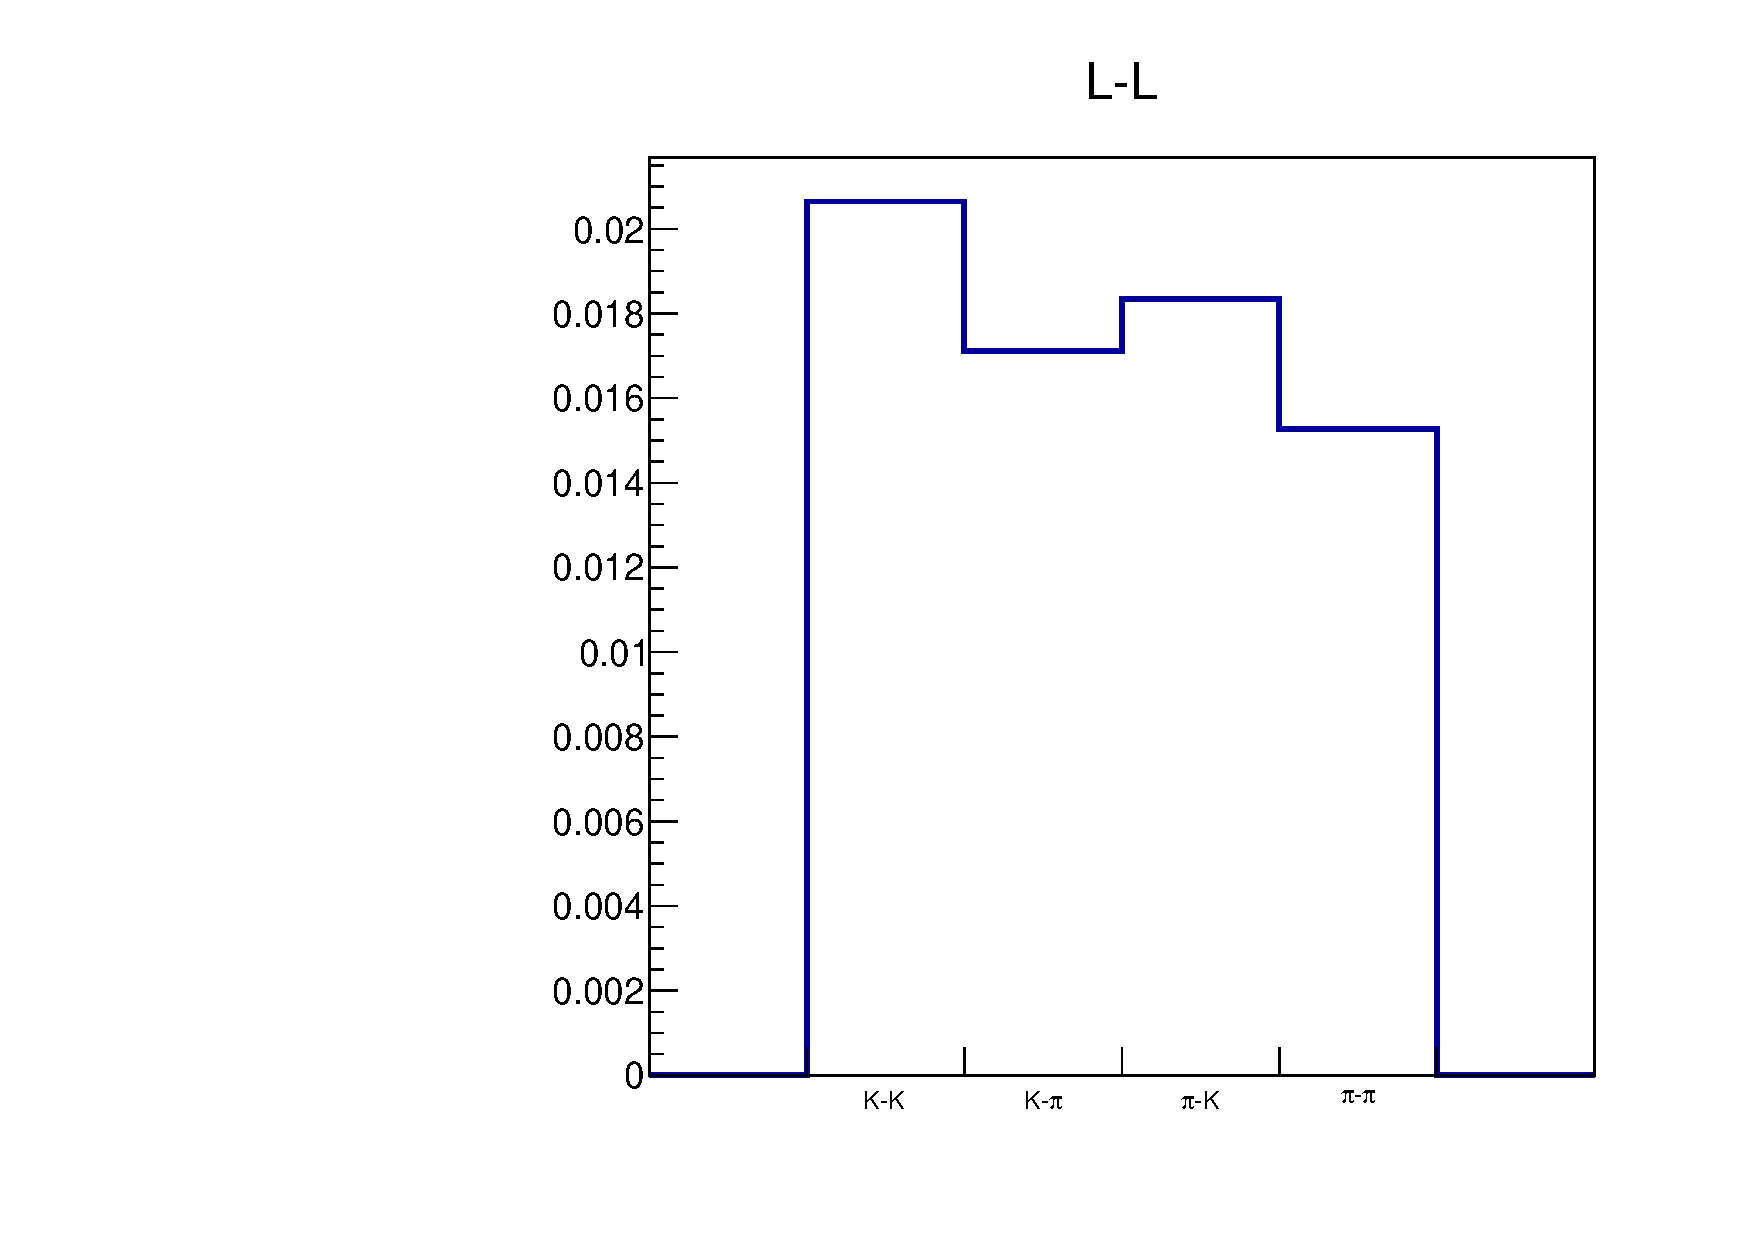
\includegraphics[width=\textwidth]{figures/FakeRatesFit/FakeRatesBhh/LL.pdf}
        \caption{Loose-Loose WP}
        \label{fig:LL}
    \end{subfigure}
    \hfill
    \begin{subfigure}[b]{0.45\textwidth}
        \centering
        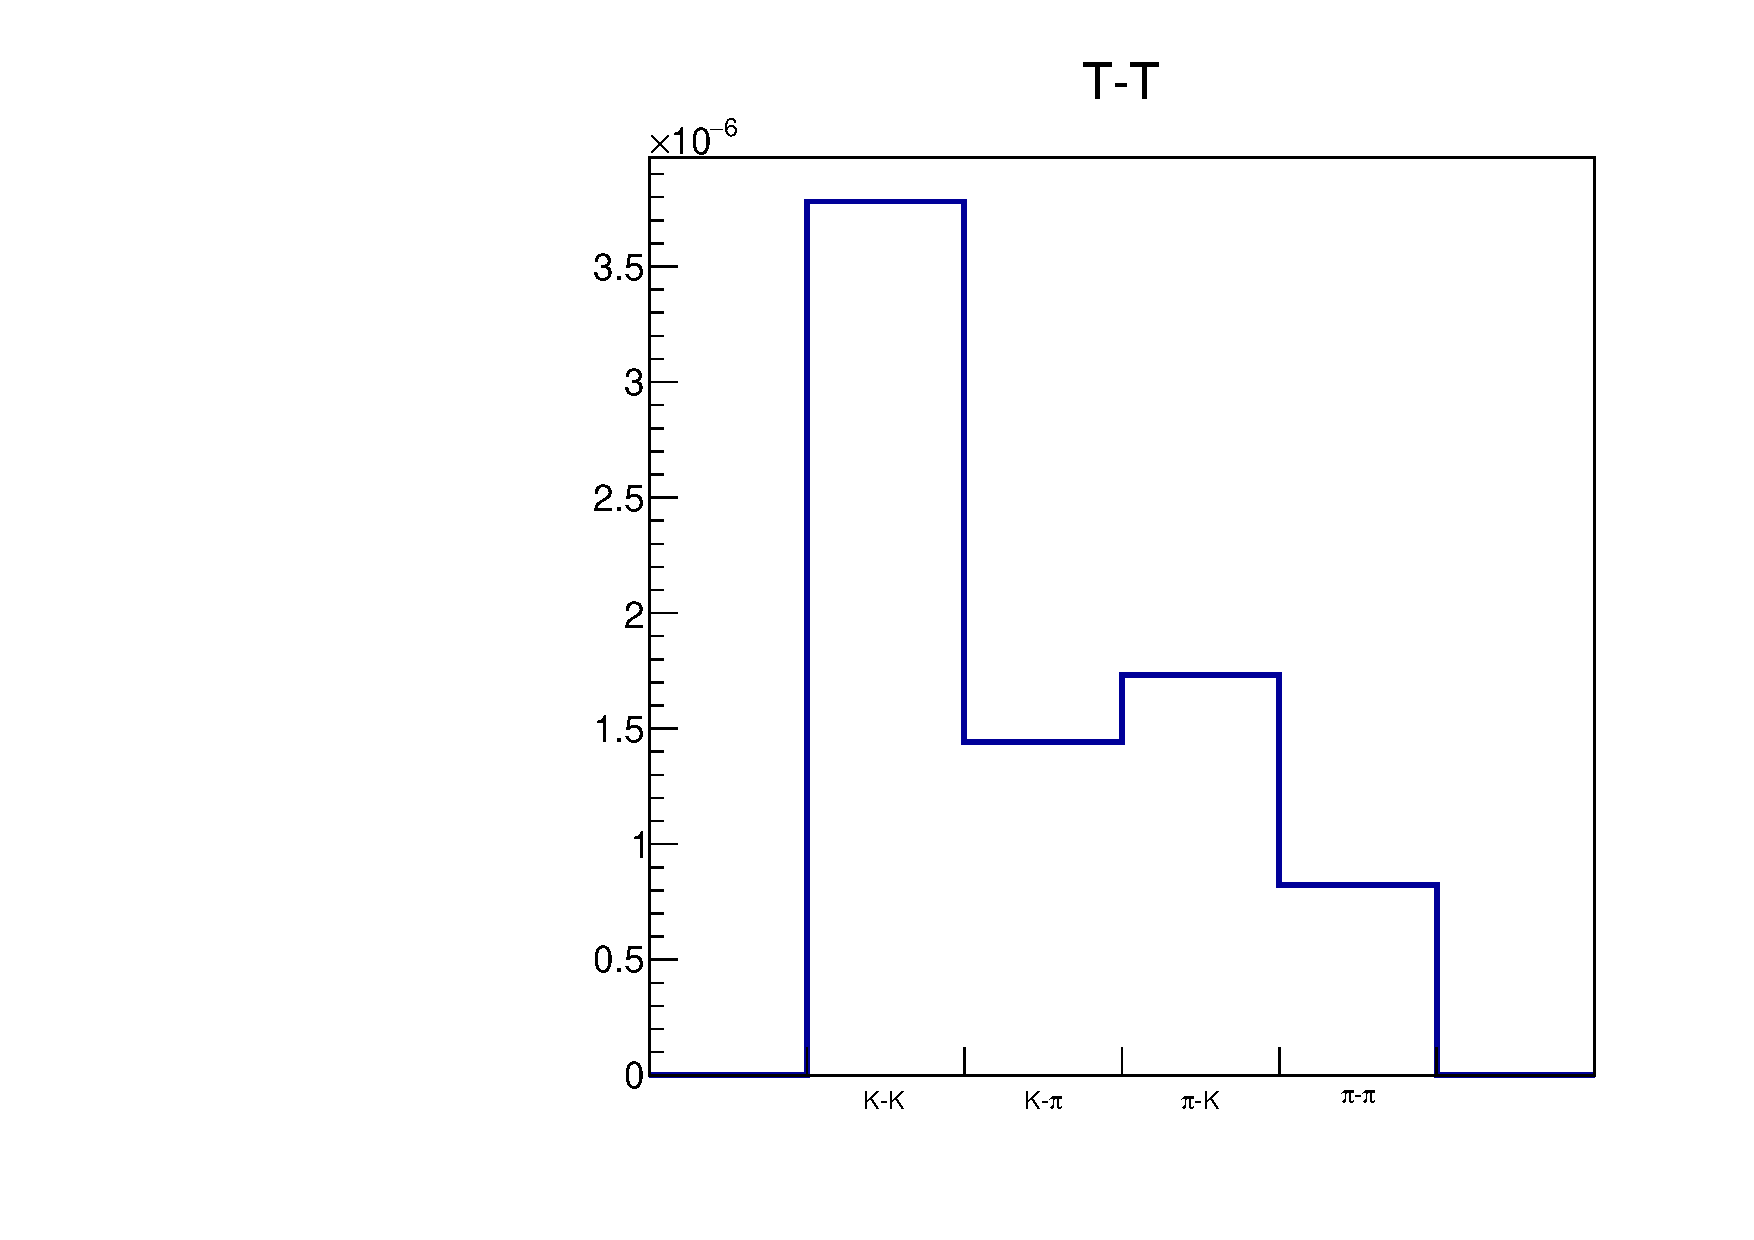
\includegraphics[width=\textwidth]{figures/FakeRatesFit/FakeRatesBhh/TT.pdf}
        \caption{Tight-Tight WP}
        \label{fig:TT}
    \end{subfigure}

    \vspace{0.5cm}
    \begin{subfigure}[b]{0.45\textwidth}
        \centering
        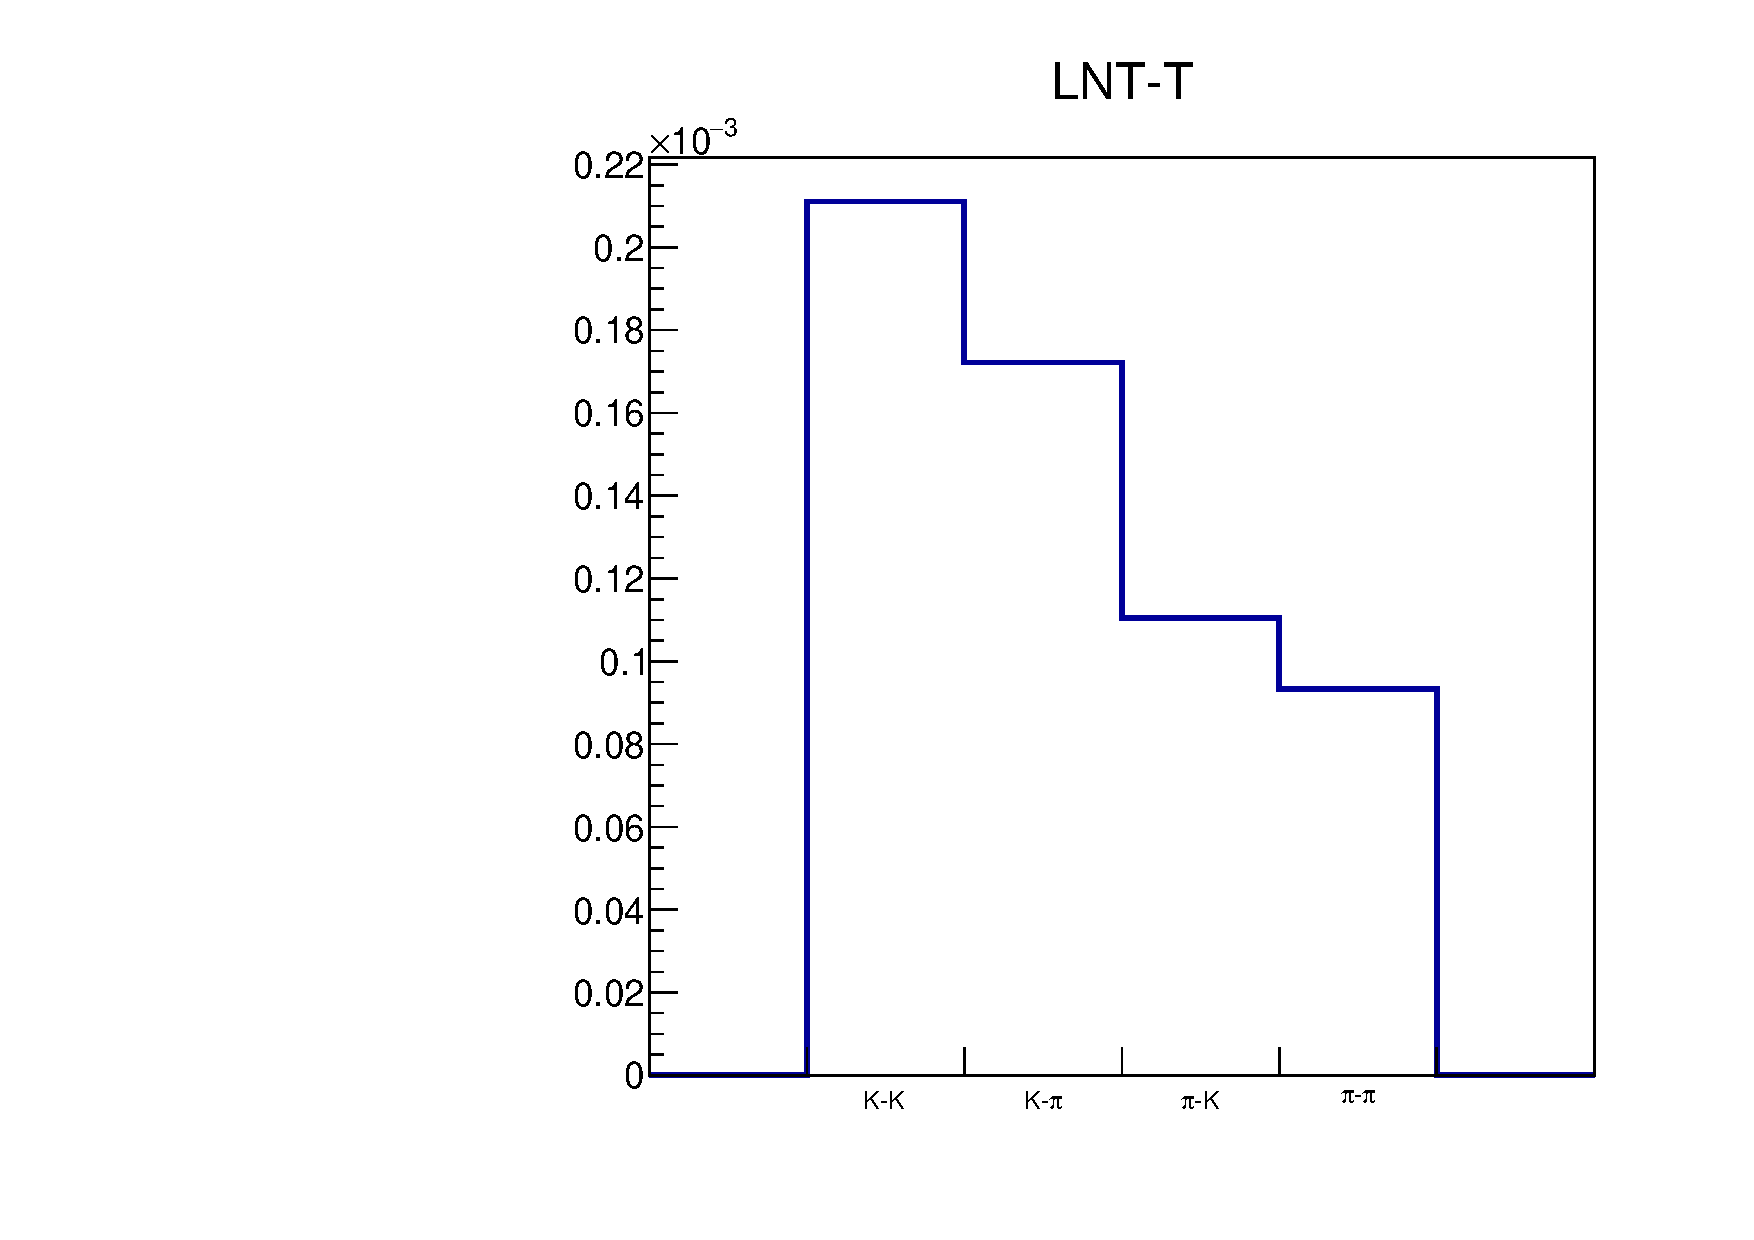
\includegraphics[width=\textwidth]{figures/FakeRatesFit/FakeRatesBhh/LNTT.pdf}
        \caption{LooseNotTight-Tight WP}
        \label{fig:LNTT}
    \end{subfigure}
    \hfill
    \begin{subfigure}[b]{0.45\textwidth}
        \centering
        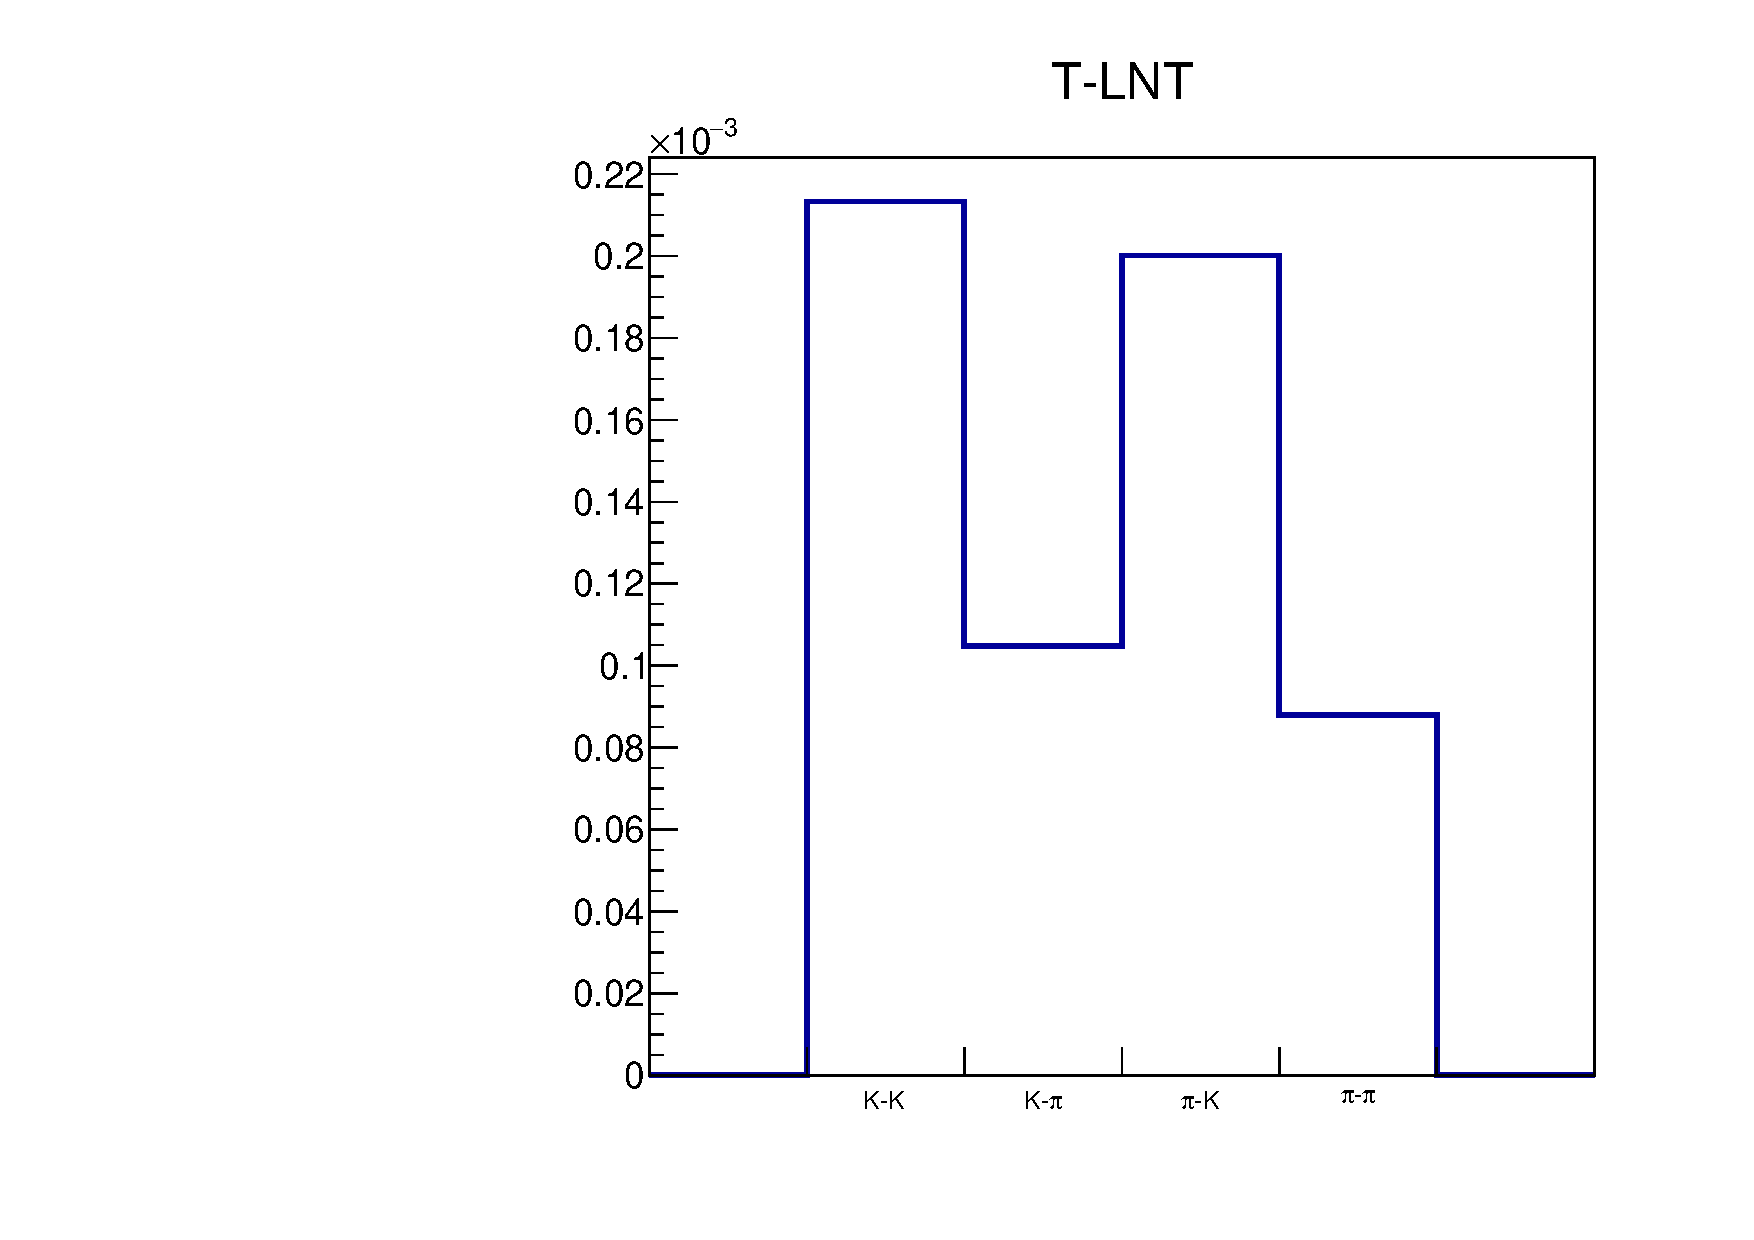
\includegraphics[width=\textwidth]{figures/FakeRatesFit/FakeRatesBhh/TLNT.pdf}
        \caption{Tight-LooseNotTight WP}
        \label{fig:TLNT}
    \end{subfigure}

    \caption{Faking rates for different Meson combinations and different WP combinations.}
    \label{fig:all_subfigures}
\end{figure}